\documentclass[oneside]{book}

% Load the VUB package.
% This has many options, please read the documentation at
% https://gitlab.com/rubdos/texlive-vub
\usepackage{vub}

%href package to make references clickable.
\usepackage{hyperref}
\hypersetup{
    colorlinks,
    citecolor=black,
    filecolor=black,
    linkcolor=black,
    urlcolor=black
}

% Some highly suggested packages, please read their manuals.
\usepackage{cleveref}
\usepackage[natbib,style=apa]{biblatex}
\addbibresource{../bibliography.bib}
\usepackage{listings}
\usepackage{wrapfig}


%smaller spacing
\usepackage{titlesec}
\titlespacing*\section{0pt}{12pt plus 4pt minus 2pt}{0pt plus 2pt minus 2pt}
\titlespacing*\subsection{0pt}{12pt plus 4pt minus 2pt}{0pt plus 2pt minus 2pt}
\titlespacing*\subsubsection{0pt}{12pt plus 4pt minus 2pt}{0pt plus 2pt minus 2pt}

%space between paragraph and indent all
\setlength{\parskip}{1em}
%\usepackage{indentfirst}



%quotes
\usepackage{epigraph}

%space between bib entries
\setlength\bibitemsep{2\itemsep}

%images settings
\graphicspath{ {./images/} }
\usepackage{graphicx,caption}
\usepackage{float}
\usepackage{rotating}
\usepackage{tikz}

% subfigures
\usepackage{subcaption}

% remove chapter text
\usepackage{titlesec}

\titleformat{\chapter}[display]
  {\normalfont\huge\bfseries}{}{0pt}{\Huge}
\titlespacing*{\chapter}
  {0pt}{0pt}{15pt}

%START title
\title{Akka Streams}
\subtitle{Assignment 1 - Software Architectures}
\author{Lennert Bontinck}
\date{Second session, 2020-2021}
\promotors{Student number: 568702}
\faculty{Computer Science: AI}
\begin{document}
\frontmatter
\maketitle
%END title


%TOC
\tableofcontents
\mainmatter

%START MAIN
\chapter{General remarks}
\label{ch:general_remarks}

%------------------------------------

\section{Notes on the assignment}
\label{sec:notes_on_ass}

None of the assignments for the Software Architectures course were submitted in the first examination period due to personal reasons.
Because of this, all of the code written for this assignment is written specifically for the second examination period.
One small \textit{bug} in the code was resolved after email communication with the teaching assistants.
This \textit{bug} and its solution will be explained later.
All other code was written by using the course material and the online Akka documentation\footnote{\url{https://akka.io/docs/}}.

%------------------------------------

\section{Important files}
\label{sec:important_files}

All code written is available on the GitHub repository for this assignment \citep{github_project}. 
Rights to this private GitHub repository can be granted upon request. 
A copy of this GitHub repository is accompanied by this report.
An overview of important files is given below:
\begin{itemize}
    \item \texttt{README.md} and \texttt{code/README.md}
    \begin{itemize}
        \item General information of the GitHub repository with \texttt{code/README.md} containing the technical details about the used environment and validated output.
    \end{itemize}
    \item \texttt{assignment.pdf} and \texttt{Lennert-Bontinck-SA1.pdf}
    \begin{itemize}
        \item The assignment PDF and this report.
    \end{itemize}
    \item \texttt{code/Lennert-Bontinck-SA1}
    \begin{itemize}
        \item The folder containing the code of the assignment solution. 
        \item \texttt{./src/main/resources/}: folder containing the input files. The results files are available under the sub-folder \texttt{./result/}.
        \item \texttt{./src/main/scala/Lennert\_Bontinck\_SA1/}: folder containing the main Scala files. Multiple files are made for separate objects and classes. All code is well documented and discussed later in this report.
    \end{itemize}
\end{itemize}


\chapter{Project defence}
\label{ch:project_defence}

In what follows the implementation details of the assignment are discussed.
Multiple figures were made to illustrate the working of different parts of the code.
A legend showing the meaning of the parts of the figure is given in figure \ref{fig:legend}.
For more technical details the reader is invited to read the comments in the code.

%------------------------------------

\section{Main application structure}
\label{sec:main_app_structure}

There are two main runnable applications: \texttt{Main} and \texttt{MainDisplay}. 
Both extend the App object and run a \texttt{RunnableGraph}.
They differ in the way they handle output by having differing sinks.
\texttt{Main} saves the output to text files in the output folder whilst \texttt{MainDisplay} prints the output to the terminal.
The former is the assignment's requirement and the latter is an easier to debug alternative.
A simplified representation of the Main application is given in figure \ref{fig:main}.
The different components will be explained in greater detail in what follows.

The most important remark to make for the main graph is the use of \texttt{alsoToMat} to reach two distinct sinks.
Alternatively, a broadcast mechanism could have been used.
These multiple sinks are required for the second term extension of the assignment, each saving a differing file.
The discussed \textit{bug} for which the teaching assistants help was received was simply the use of \texttt{to} instead of \texttt{toMat} for flowing to the sink, causing premature termination of the graph.  

\begin{figure}[H]
    \centering
    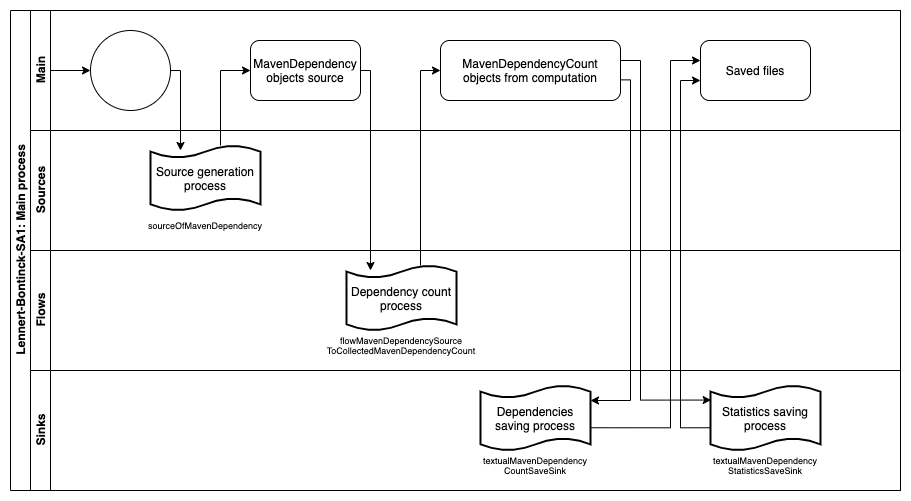
\includegraphics[width=0.8\linewidth]{images/main.png}
    \captionsetup{width=0.7\linewidth}
    \captionsetup{justification=centering}
    \caption{Simplified representation of the main application.  }
    \label{fig:main}
\end{figure}





%------------------------------------

\section{MD, MDC and MDS objects}
\label{sec:MD_vs_MDC_vs_MDS}

There are a total of three case classes for this assignment.
\texttt{MavenDependency} (\texttt{MD}) represents a singular Maven dependency as instantiated from the extracted file.
It has a \texttt{library} (name), \texttt{dependency} and \texttt{dependency\_type}. 
Thus multiple dependencies of an equal Maven library give rise to different \texttt{MD} objects.
Its companion object provides an alternative constructor.

\texttt{MavenDependencyCount} (\texttt{MDC}) represents a Maven library and its dependencies.
It has a \texttt{library} (name) and a dependency count per dependency type (\texttt{compile}, \texttt{provided}, \texttt{runtime} and \texttt{test}).
Its companion object provides a function for combining two \texttt{MDC} objects.
The \texttt{MavenDependencyStatistics} (\texttt{MDS}) object is used for the statistics part of the assignment.
It has a \texttt{minimumDependencies} and a count of libraries eligible for the statistic per dependency type.
Its companion object provides a function for adding a \texttt{MDC} object to the statistic object.


%------------------------------------

\section{Source generation process}
\label{sec:source_gen_proc}

Figure \ref{fig:main} shows how \texttt{Main} makes use of a source generation process to provide a list of \texttt{MD} objects as source.
This source is available as \texttt{sourceOfMavenDependency} under the \texttt{Sources} object.
The process of generating this source is visualised in figure \ref{fig:source}.

The process makes use of an initial \texttt{ByteString} source which is simply the extracted file.
The raw \texttt{ByteString} source is then parsed as a CSV through \texttt{CsvParsing} whose records are then converted to a map of strings.
This map can be used to instantiate \texttt{MD} objects resulting in a source of \texttt{MD} objects.

\begin{figure}[H]
    \centering
    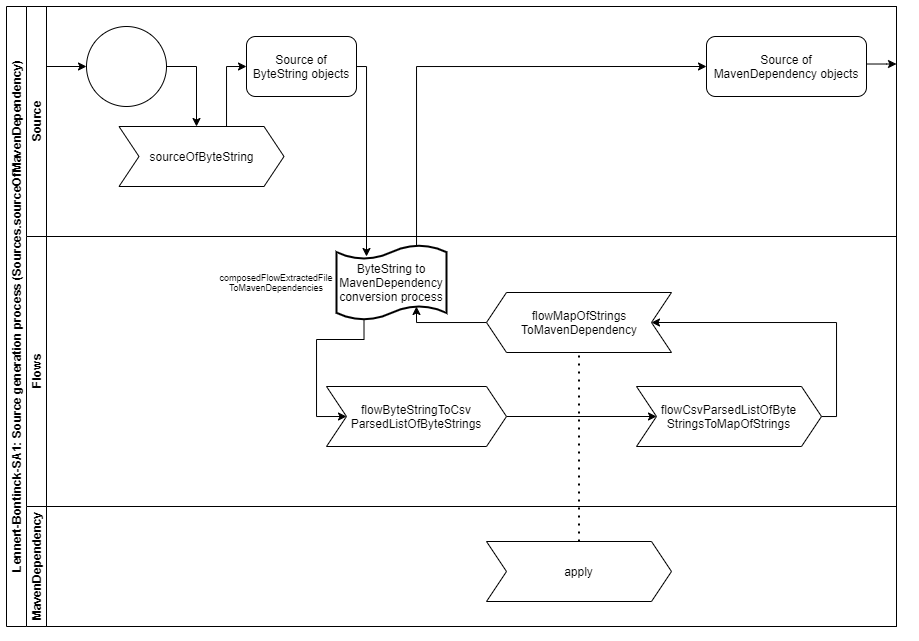
\includegraphics[width=0.85\linewidth]{images/source.png}
    \captionsetup{width=0.8\linewidth}
    \captionsetup{justification=centering}
    \caption{Simplified representation of the source generation process.  }
    \label{fig:source}
\end{figure}




%------------------------------------

\section{Source generation process}
\label{sec:source_gen_proc}

Figure \ref{fig:main} shows how \texttt{Main} makes use of the explained \texttt{MD} object source to collect \texttt{MDC} objects through a dependency count process.
This dependency count process is available as \texttt{flowMavenDependencySource\-ToCollectedMavenDependencyCount} under the \texttt{Flows} object.
This flow makes use of custom flow shapes and is visualised in figure \ref{fig:counting}.

First, the incoming stream of \texttt{MD} objects is grouped on their library name to create a substream for each library.
\texttt{flowMavenDependency\-ToMavenDependencyCount\-Parallel} is a custom flow shape responsible for making a balanced approach of counting the dependencies by adding a \texttt{Balance\-[MavenDependency]} having two ports.
These two ports then perform the same custom flow shape \texttt{flowMavenDependencyToMavenDependencyCount} to perform the actual counting and are merged on the end.
All of this is included in \texttt{flow\-Maven\-Dependency\-To\-Maven\-Dependency\-Count\-Parallel}.

\texttt{flowMavenDependencyToMavenDependencyCount} is shown in detail.
The counting happens by broadcasting the incoming \texttt{MD} objects to four separate flows.
These flows generate \texttt{MDC} objects having either a count of one or zero for the field they are counting.
All of these \texttt{MDC} objects are then merged to a singular \texttt{MDC} object by using \texttt{toSingleMavenDependencyCount}, which uses \texttt{flowMultipleMavenDependencyCountsToSingle} which in it turns uses \texttt{merge\-Maven\-Dependency\-Count} from the \texttt{MDC} companion object. 

\begin{figure}[H]
    \centering
    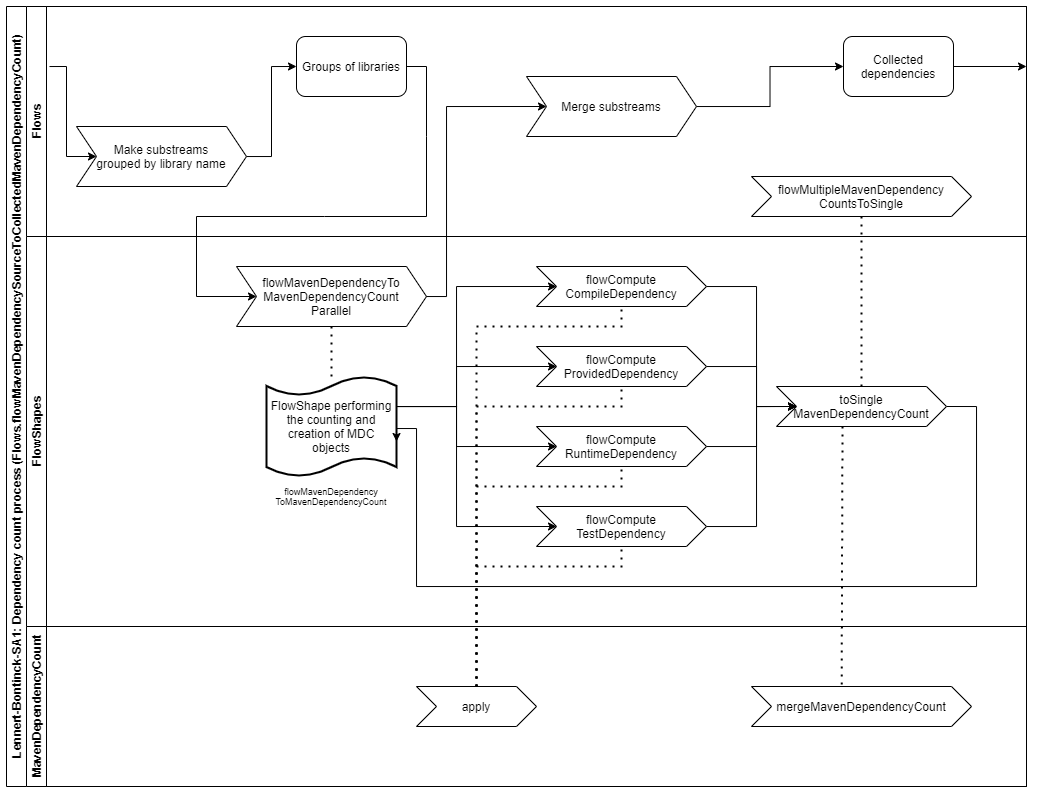
\includegraphics[width=0.95\linewidth]{images/counting.png}
    \captionsetup{width=0.7\linewidth}
    \captionsetup{justification=centering}
    \caption{Simplified representation of the counting process.  }
    \label{fig:counting}
\end{figure}




%------------------------------------

\section{Saving process}
\label{sec:sink_proc}

Figure \ref{fig:main} shows how \texttt{Main} makes use of the explained \texttt{MDC} objects to save dependency count and statistical information to a text file.
This saving process is available as the \texttt{textual\-Maven\-Dependency\-Count\-Save\-Sink} and \texttt{textualMavenDependencyStatisticsSaveSink} sink under the \texttt{Sinks} object.
Figure \ref{fig:counting} visualises the saving process.

Saving consists of generating the right \texttt{ByteString} stream which can then be saved by \texttt{FileIO.toPath}.
For the first sink, this just consists of converting each input \texttt{MDC} object to a textual representation in the specified form.
For the second sink, the input \texttt{MDC} objects need conversion to \texttt{MDS} objects first before the specified textual representation can be made.
In order to do this, the function \texttt{mergeMavenDependencyCount} from the companion object of the \texttt{MDS} class can be used in a folding manner.
This is done in \texttt{flow\-MavenDependency\-Count\-To\-Maven\-Dependency\-Statistics} where \texttt{minimumDependencies} can also be specified.


\begin{figure}[H]
    \centering
    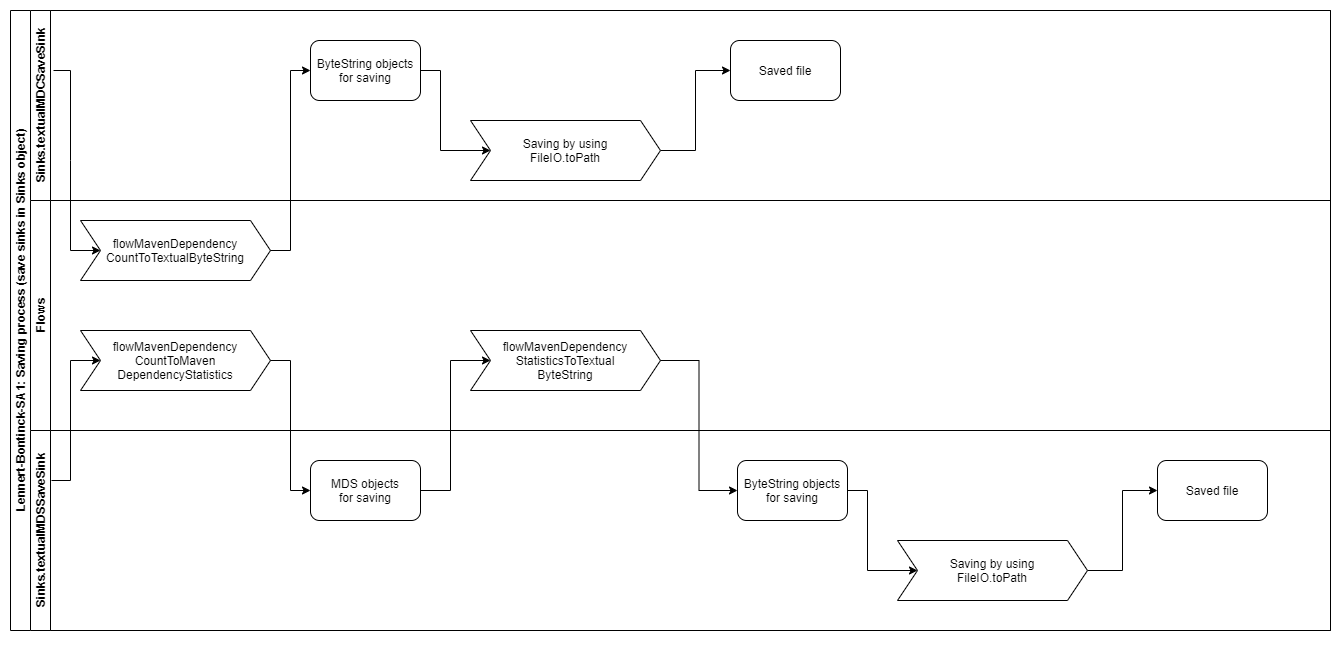
\includegraphics[width=0.95\linewidth]{images/sinks.png}
    \captionsetup{width=0.7\linewidth}
    \captionsetup{justification=centering}
    \caption{Simplified representation of the saving process. }
    \label{fig:sinks}
\end{figure}

\begin{figure}[H]
    \centering
    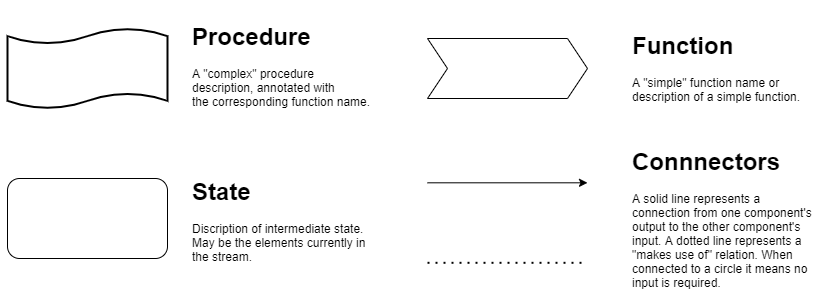
\includegraphics[width=0.95\linewidth]{images/legend.png}
    \captionsetup{width=0.7\linewidth}
    \captionsetup{justification=centering}
    \caption{Legend for the figures. }
    \label{fig:legend}
\end{figure}

%references list
\nocite{*}
\printbibliography[heading=bibintoc, title={References}]
\end{document}
